\documentclass[a4paper,11pt]{article}
\usepackage{geometry}
\usepackage{amsmath, amssymb}
\usepackage{xcolor}
\usepackage[most]{tcolorbox}
\usepackage{multicol}
\usepackage{enumitem}
\usepackage{tasks}  % pour lister des items en colonnes
\usepackage{yhmath}
\usepackage{listing}
\usepackage{graphicx}% pour \includegraphics
\usepackage{tikz}
\usepackage{color}
\usepackage{makecell}
\usepackage{fancyhdr}
\usepackage{lastpage}
\usepackage{currfile}
\usepackage[skip=8pt plus1pt, indent=0pt]{parskip}

\graphicspath{ {../Images/} }
\input{\currfiledir ../def.tex}

\usetikzlibrary{calc,angles,quotes}
% Définition de la "pic" "tick"
\tikzset{
  pics/tick/.style args={#1}{
    code={
      % "#1" correspond à la longueur du tick.
      \draw[line width=1pt, line cap=round] (-#1/2,0) -- (#1/2,0);
    }
  }
}

\definecolor{mygreen}{rgb}{0,0.6,0}
\definecolor{mygray}{rgb}{0.5,0.5,0.5}
\definecolor{mymauve}{rgb}{0.58,0,0.82}
\definecolor{mywhite}{rgb}{0.9,0.9,0.9}
\renewcommand{\thefootnote}{\arabic{footnote}}

\newcommand{\footnotettfamily}{\ttfamily\footnotesize}

\newcommand{\scriptttfamily}{\ttfamily\scriptsize}

\lstset{ %
  backgroundcolor=\color{mywhite},   % choose the background color
  basicstyle=\ttfamily\scriptttfamily,
  breaklines=true,                 % automatic line breaking only at whitespace
  captionpos=b,                    % sets the caption-position to bottom
  commentstyle=\color{mygreen},    % comment style
  escapeinside={\%*}{*)},          % if you want to add LaTeX within your code
  keywordstyle=\color{blue},       % keyword style
  stringstyle=\color{mymauve},     % string literal style
}

\graphicspath{ {../Images/} } % chemin vers le dossier d'images
\hyphenpenalty=10000

\geometry{left=1cm, right=1cm, top=2cm, bottom=2cm}

\tcbuselibrary{theorems}

\definecolor{PurpleEx}{HTML}{5d478b}
\definecolor{GrayEx}{HTML}{f2f2f2}
\definecolor{GrayBG}{HTML}{d9d9d9}
\definecolor{BlackSav}{HTML}{000000}
\definecolor{RedMet}{HTML}{cd5556}

%\title{
%\vspace{-3em}
%\centering
%\tcbset{colframe=BlackSav,colback=GrayBG}
%\tcbox[tikznode]{
%  Exercices \\ Tableaux croisés et probabilités conditionnelles
%}
%}
%\author{}
%\date{}

\newtcbtheorem
[]% init options
{exercice}% name
{Exercice}% title
{%
colback=GrayEx,
colframe=PurpleEx,
fonttitle=\bfseries,
breakable=true,
parbox=false,
before upper={\renewcommand{\thempfootnote}{\arabic{mpfootnote}}}
}% options
{ex}% prefix


\begin{document}

\pagestyle{fancy}

\fancyhf{} % clear existing header/footer entries
\fancyhead[R]{ {\Niveau}}
\fancyhead[L]{ {\Chapitre}}
%\fancyhead[R]{\large \textbf{\textbf{\Document\ (B) -- 1h}}}
\fancyfoot[L]{ A. Fernandez }
\fancyfoot[R]{{\thepage\  / \pageref{LastPage}}}


\begin{multicols}{2}

\begin{exercice}[title=Exercice 1 $\star$ { [Calculer, Représenter] }]{}{}
  L'association sportive d'un lycée compte 240 adhérents parmi lesquels il y a 130 demi-pensionnaires, les autres adhérents étant externes. Ces adhérents doivent choisir un sport et un seul parmi les trois proposés : le basket-ball, le volley-ball, et la natation.
  
  \begin{enumerate}
    \item On sait que $30\%$ des adhérents ont choisi le volley-ball. Vérifier que 72 adhérents ont choisi le volley-ball.
    \item On sait que $25\%$ des adhérents sont des demi-pensionnaires ayant choisi la natation. Calculer le nombre d'adhérents demi-pensionnaires ayant choisi la natation.
    \item On sait de plus que :
      \begin{itemize}[label=$\bullet$]
        \item 66 adhérents ont choisi le basket-ball ;
        \item 40 adhérents pratiquent le volley-ball et sont demi-pensionnaires.
      \end{itemize}
      Recopier et compléter le tableau suivant :
      
  \end{enumerate}
      \begin{center}
      \small
      \renewcommand{\arraystretch}{1.2}
      \begin{tabular}{|c|c|c|c|c|}
      \hline
       & \makecell{Basket-\\ball} & \makecell{Volley-\\ball} & Natation & Total \\ \hline
      \makecell{Demi-\\pensionnaires} & & 40 & & \\ \hline
      Externes & & & & \\ \hline
      Total & 66 & & & 240 \\ \hline
      \end{tabular}
      \end{center}
\end{exercice}

\null\vfill

\begin{exercice}[title=Exercice 2 $\star$ { [Calculer, Représenter] }]{}{}
  Alice fabrique chaque semaine 250 bijoux fantaisie qu'elle vend en fin de semaine. Sa production hebdomadaire de bijoux se répartit comme suit : $20\%$ de boucles d'oreilles, $40\%$ de colliers et $40\%$ de bracelets.
  
  Chaque bijou est réalisé, soit en métal argenté, soit en métal doré. $60\%$ des bijoux fabriqués sont argentés.
  Elle fabrique autant de colliers argentés que de colliers dorés. $75\%$ des bracelets sont argentés.
  
  Compléter le tableau suivant :
  
  \begin{center}
  \small
  \renewcommand{\arraystretch}{1.2}
  \begin{tabular}{|c|c|c|c|c|}
  \hline
   & Collier & Bracelet & \makecell{Boucles \\d'oreilles} & Total \\ \hline
  Argenté & & & & \\ \hline
  Doré & & & & \\ \hline
  Total & & & & 250 \\ \hline
  \end{tabular}
  \end{center}
\end{exercice}

\newcolumn

\begin{exercice}[title=Exercice 3 $\star$ { [Calculer] }]{}{}
  On donne ci-dessous le tableau croisé d'effectifs d'un ensemble de jetons classés suivant leur forme et leur couleur.
  
  \begin{center}
  \small
  \renewcommand{\arraystretch}{1.2}
  \begin{tabular}{|c|c|c|c|}
  \hline
   & Carré & Triangle & Total \\ \hline
  Rouge & 30 & 20 & 50 \\ \hline
  Vert & 10 & 40 & 50 \\ \hline
  Total & 40 & 60 & 100 \\ \hline
  \end{tabular}
  \end{center}
  
  \begin{enumerate}[noitemsep]
    \item 
      \begin{enumerate}[noitemsep]
        \item[(a)] Quel est le nombre total de jetons ?
        \item[(b)] Quel est le nombre total de jetons carrés ?
        \item[(c)] En déduire la fréquence des jetons carrés.
      \end{enumerate}
    \item Calculer la fréquence des jetons verts.
    \item Parmi tous les jetons, quel est le pourcentage de jetons rouges et carrés ?
  \end{enumerate}
\end{exercice}


\begin{exercice}[title=Exercice 4 $\star$ { [Calculer] }]{}{}
  Voici la répartition des candidats au BTS à la session 2017 (en milliers) selon la spécialité :
  
  \begin{center}
  \small
  \renewcommand{\arraystretch}{1.2}
  \begin{tabular}{|c|c|c|c|}
  \hline
   & Hommes & Femmes & Total \\ \hline
  Production & & 11 & 54 \\ \hline
  Service & & & 126 \\ \hline
  Total & 88 & 92 & 180 \\ \hline
  \end{tabular}
  \end{center}
  
  \begin{enumerate}[noitemsep]
    \item Compléter le tableau.
    \item Parmi les candidats au BTS, quelle est la proportion de femmes ?
    \item Calculer la fréquence de la spécialité ``Production''.
  \end{enumerate}
\end{exercice}



\begin{exercice}[title=Exercice 5 $\star$ { [Calculer] }]{}{}
  On donne dans le tableau ci-dessous la répartition des 200 élèves de Première technologique d'un lycée selon leur sexe et leur régime.
  
  \begin{center}
  \small
  \renewcommand{\arraystretch}{1.2}
  \begin{tabular}{|c|c|c|c|}
  \hline
   & Filles & Garçons & Total \\ \hline
  Externes & 40 & 20 & 60 \\ \hline
  Demi-pensionnaires & 60 & 40 & 100 \\ \hline
  Internes & 20 & 20 & 40 \\ \hline
  Total & 120 & 80 & 200 \\ \hline
  \end{tabular}
  \end{center}
  
  \begin{enumerate}[noitemsep]
    \item Quelle est la fréquence de filles ?
    \item Quelle est la proportion d'externes ?
    \item 
      \begin{enumerate}[noitemsep]
        \item[(a)] Combien y a-t-il d'internes en tout ?
        \item[(b)] Parmi les internes, combien y a-t-il de filles ?
        \item[(c)] En déduire la proportion de filles parmi les internes.
      \end{enumerate}
  \end{enumerate}
\end{exercice}

\null\vfill

\begin{exercice}[title=Exercice 6 $\star$ { [Calculer] }]{}{}
  On donne la répartition des élèves de Première et de Terminale d'un lycée :
  
  \begin{center}
  \small
  \renewcommand{\arraystretch}{1.2}
  \begin{tabular}{|c|c|c|c|}
  \hline
   & Générale & Technologique & Total \\ \hline
  Première & 100 & 175 & 275 \\ \hline
  Terminale & 150 & 75 & 225 \\ \hline
  Total & 250 & 250 & 500 \\ \hline
  \end{tabular}
  \end{center}
  
  \begin{enumerate}
    \item Quel est le nombre de lycéens en filière Générale ?
    \item Quel est le nombre de lycéens en classe de Première Générale ?
    \item En déduire la fréquence des lycéens en Première parmi ceux de filière Générale.
    \item Déterminer la fréquence des lycéens en filière Technologique parmi les Terminales.
  \end{enumerate}
\end{exercice}

\null\vfill

\begin{exercice}[title=Exercice 7 $\star$ { [Représenter, Calculer] }]{}{}
  Une association sportive interroge 100 élèves sur leur pratique sportive et leur sexe/établissement. Les résultats sont les suivants :
  \begin{itemize}[label=$\bullet$]
    \item 40 collégiens font du sport en club.
    \item 10 lycéens font du sport en club.
    \item 30 lycéens ne font pas de sport.
    \item 20 collégiens ne font pas de sport.
  \end{itemize}
  
  \begin{enumerate}
    \item Construire un tableau croisé d'effectifs correspondant à la situation \footnote{(\emph{Aide :} on mettra en ligne l'établissement — collège ou lycée — et en colonnes la pratique sportive)}.
    \item Quelle est la proportion d'élèves ne faisant pas de sport en club ?
    \item Calculer le pourcentage de collégiens parmi les élèves pratiquant le sport en club.
  \end{enumerate}
\end{exercice}


\newcolumn

\begin{exercice}[title=Exercice 8 $\star\star$ { [Représenter, Calculer] }]{}{}
  Le parc informatique d'un lycée est composé de 200 ordinateurs. 30 sont considérés comme neufs ; 90 sont considérés comme récents et les autres sont considérés comme anciens.
  
  Une étude statistique indique qu'aucun ordinateur neuf n'est défaillant ; $10\%$ des ordinateurs récents sont défaillants et $25\%$ des ordinateurs anciens sont défaillants.
  
  \begin{enumerate}
    \item Traduire l'énoncé par un tableau croisé d'effectifs.
    \item On choisit au hasard un ordinateur de ce parc informatique. Déterminer la probabilité que l'ordinateur soit ancien sachant qu'il est défaillant.
  \end{enumerate}
\end{exercice}


\null\vfill

\begin{exercice}[title=Exercice 9 $\star\star$ { [Calculer] }]{}{}
  On a représenté deux ensembles $A$ et $B$ ainsi que leurs cardinaux. On tire au hasard l'un des éléments.
  
  \begin{center}
  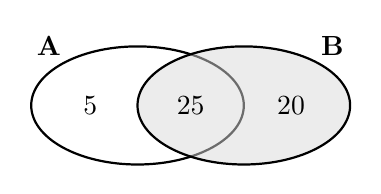
\begin{tikzpicture}[scale=0.75]
    \draw[thick] (0,0) ellipse (1.8cm and 1cm);
    \draw[thick, fill=gray!30, fill opacity=0.5] (1.8,0) ellipse (1.8cm and 1cm);
    \node at (-0.8,0) {5};
    \node at (0.9,0) {25};
    \node at (2.6,0) {20};
    \node at (-1.5,1) {\textbf{A}};
    \node at (3.3,1) {\textbf{B}};
  \end{tikzpicture}
  \end{center}
  
  \begin{enumerate}
    \item Calculer $\mathrm{Card}(A)$, $\mathrm{Card}(A \cup B)$ et $\mathrm{Card}(A \cap B)$.
    \item Calculer $P_B(A)$.
  \end{enumerate}
\end{exercice}

\null\vfill

\begin{exercice}[title=Exercice 10 $\star\star$ { [Chercher, Modéliser] }]{}{}
  On lance deux fois un dé non truqué à six faces et on considère le nombre formé par les deux numéros pris dans l'ordre de sortie. Par exemple, si l'on obtient 5 et 6 pour les deux lancers, on considère le nombre 56.

  \begin{enumerate}[noitemsep]
    \item Calculer la probabilité que le nombre considéré soit premier sachant qu'il contient au moins un 2.
    \item Calculer la probabilité que le nombre considéré contienne au moins un 3 sachant qu'il est premier.
  \end{enumerate}
\end{exercice}

\null\vfill

\newcolumn

\begin{exercice}[title=Exercice 11 $\star\star$ { [Raisonner, Calculer] }]{}{}
  \emph{D'après le sujet zéro.} \\
  Indiquer, en justifiant, si les affirmations suivantes sont vraies ou fausses.
  
  Afin de lutter contre le dopage dans le sport, un test a été mis en place. En principe, ce test est POSITIF lorsque le sportif est dopé, et NÉGATIF lorsqu'il n'est pas dopé. Toutefois, ce test peut commettre des erreurs : il peut être positif lorsque le sportif n'est pas dopé, et négatif lorsque le sportif est dopé.
  
  Le tableau ci-dessous donne les résultats recueillis auprès de 200 coureurs ayant participé à un marathon :
  
  \begin{center}
  \small
  \renewcommand{\arraystretch}{1.2}
  \begin{tabular}{|c|c|c|c|}
  \hline
   & \makecell{Coureur \\non dopé} & \makecell{Coureur \\dopé} & Total \\ \hline
  Test positif & 15 & 5 & 20 \\ \hline
  Test négatif & 178 & 2 & 180 \\ \hline
  Total & 193 & 7 & 200 \\ \hline
  \end{tabular}
  \end{center}
  
  \begin{enumerate}
    \item[(a)] On choisit un coureur au hasard parmi les 200 coureurs testés. \\
    \textbf{Affirmation 1 :} La probabilité que le coureur ne soit pas dopé ou soit testé positif est égale à $\dfrac{213}{200}$.
    
    \item[(b)] On choisit un coureur au hasard parmi ceux ayant eu un test positif. \\
    \textbf{Affirmation 2 :} Il y a $75\%$ de chances que le coureur ne soit pas dopé.
    
    \item[(c)] On choisit un coureur au hasard parmi les 200 coureurs testés. \\
    \textbf{Affirmation 3 :} La probabilité que le coureur soit concerné par une erreur de test est égale à $8{,}5\%$.
  \end{enumerate}
\end{exercice}

\newcolumn

\begin{exercice}[title=Exercice 12 $\star\star$ { [Modéliser, Calculer] }]{}{}
  Une enquête est réalisée auprès des 1\,200 élèves du lycée Bourbaki qui possèdent un téléphone portable afin de connaître le type d'appareil et le type de forfait dont ils disposent.
  Il en ressort que : 200 élèves possèdent un smartphone et parmi eux $20\%$ ont un forfait bloqué. Au total, 360 élèves ont un forfait non bloqué.

  \begin{enumerate}
    \item Recopier et compléter le tableau ci-dessous~:
  \end{enumerate}
      \begin{center}
      \small
      \renewcommand{\arraystretch}{1.2}
      \begin{tabular}{|c|c|c|c|}
      \hline
       & \makecell{Possède un\\smartphone} & \makecell{Possède un\\autre téléphone} & Total \\ \hline
      \makecell{Forfait \\bloqué} & & & \\ \hline
      \makecell{Forfait \\non bloqué} & & & 360 \\ \hline
      Total & 200 & & 1\,200 \\ \hline
      \end{tabular}
      \end{center}

  On interroge au hasard un élève du lycée Bourbaki et on considère les événements :
  \begin{itemize}[label=$\bullet$]
    \item $S$ : « l'élève interrogé a un smartphone » ;
    \item $B$ : « l'élève interrogé a un forfait bloqué ».
  \end{itemize}

  \begin{enumerate}[resume]
    \item Calculer la probabilité de l'événement $B$ et celle de l'événement $S$.
    \item L'élève interrogé a un smartphone. Quelle est la probabilité qu'il ait un forfait non bloqué ?
    \item Décrire par une phrase l'événement $S \cup B$ et calculer la probabilité de cet événement.
  \end{enumerate}
\end{exercice}



\begin{exercice}[title=Exercice 13 $\star\star\star$ { [Modéliser, Calculer, Communiquer] }]{}{}
  Le dépistage d'une maladie s'effectue par un test basé sur le dosage d'une hormone particulière. On estime qu'elle touche environ \(1\%\) d'une population de 100 000 personnes.

  Un de vos amis a été diagnostiqué positif à cette maladie. Le médecin lui a indiqué que pour une personne atteinte par la maladie, le test est positif dans \(95\%\) des cas, alors que pour une personne non atteinte, le test est négatif dans \(85\%\) des cas.

  Comment pouvez-vous rassurer votre ami ? (On cherchera à calculer la probabilité qu'il soit réellement malade sachant que son test est positif).
\end{exercice}


\null\vfill

\end{multicols}

\end{document}